\subsection{Criteria}\label{sec:architecturecriteria}
A good software system is one that meets its requirements and has no major weaknesses \citep[p.~179]{Rod-Aalborg}.
This system's requirements are listed and prioritized in \cref{sec:requirements} and the efforts put into avoiding weaknesses are laid out in this section.

Due to the conditions this system is developed under, flaws are to be expected.
%Anna:Which conditions are we talking about?
To minimize the amount of critical flaws the criteria \citep[p.~180]{Rod-Aalborg} upon which the system will be judged have been prioritized.
%Anna: burde referencen ikke stå sidst i den sætning?
The idea is that development will be focused on the 'very important' and 'important' criteria to make sure that all of these work.
Less effort will be put into the 'less important', 'irrelevant' or 'easily fulfilled' criteria, making flaws in these areas more likely.
%Anna: Evt skrive "opening more up for the likelyhood of mistakes",  "easily fulfilled burde den være kategoriseret på den måde altså at det er mulighed for flere fejl ? (hvis det er easily fulfilled burde der ikke være fejl i det)
However, as established they are less important and therefore the flaws will most likely not be critical.
%Anna: det at fejlene ikke er critical, most likely burde det ikke være noget hvor man analysere hvilke typer fejl der kan komme og derefter vurderer dem som ikke critical??? (Spørgsmål stillet i uvidenhed)
These priorities can be found in \cref{fig:criteria} and the reasoning behind them follows below.


%\begin{figure}[H]
%	\centering
%	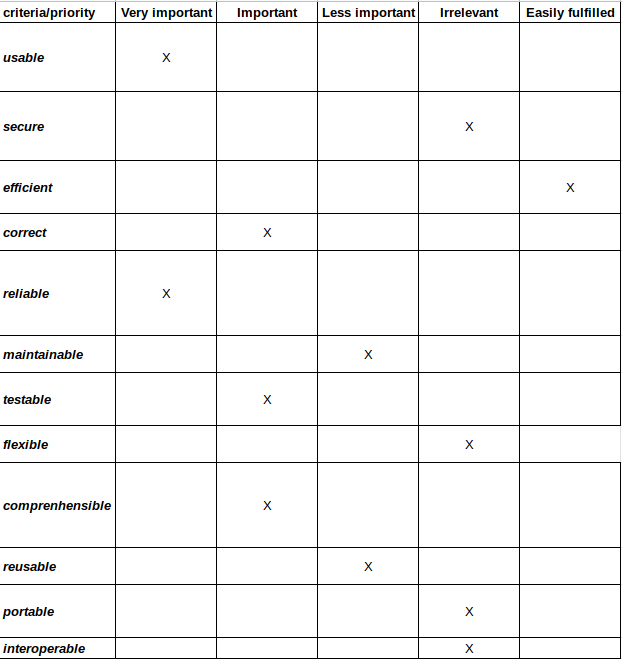
\includegraphics[width=1\textwidth]{billeder/architecture-priorities.png}
%	\caption{\textit{Prioritized list
%	}\label{fig:criteria}}
%\end{figure}
%Anna: Har lavet figuren om til en tabel nedenfor

\begin{table}[H]
	\begin{center}
		\begin{tabular}{|l|c|c|c|c|c|}
			\hline
			Criteria $\backslash$ priority & \rotatebox{90}{Very important} &  \rotatebox{90}{Important} & \rotatebox{90}{Less important} & \rotatebox{90}{Irrelevant} & \rotatebox{90}{Easily fulfilled}\\
			\hline
			Usable & \xmark & & & & \\
			\hline
			Secure & & & & \xmark & \\
			\hline
			Efficient & & & & & \xmark \\
			\hline
			Correct & & \xmark & & & \\
			\hline
			Reliable & \xmark & & & & \\
			\hline
			Maintainable & & & \xmark & & \\
			\hline
			Testable & & \xmark & & & \\
			\hline
			Flexible & & & & \xmark & \\
			\hline
			Comprehensible & & \xmark & & & \\
			\hline
			Reusable & & & \xmark & & \\
			\hline
			Portable & & & & \xmark & \\
			\hline
			Interoperable & & & & \xmark & \\
			%Anna: Hvad betyder det(er det stavet rigtigt)?
			\hline
		\end{tabular}
	\end{center}
	\caption{Prioritized list}\label{fig:criteria}
\end{table}


It is very important that the system is \textbf{usable}. 
It is assumed that the system will mainly have one user: The administrator. 
This fact could make this criterion less critical, however it is also assumed that this one user will have limited IT experience. 
Moreover this system is developed specifically for that one specific user and it is therefore imperative that they are able to use the system.
%Anna: er det ikke en yderst forkert påstand, system understøtter jo af en grund 3 forskellige typer af brugere, og selv inden for administratoren er der både kvalitetschefen og som regel sekretæren (hvor sekretæren vil tage sig af at oprette brugerne i systemet, og kvalitetschefen varetager håndbogen) men de enkelt edepartmentheads kan man jo også opleve skal arbejde med det.
%Anna (fortsat): Er princippet ikke at det skal være usable fordi det skal være lige til at konvertere til (skal ikke bruges til på at sætte sig ind i det nye system, mere end højest nødvendigt) og fordi flere af brugerne netop kan opleves at have limited experience?

The user has expressed that whether or not the system is \textbf{secure} is no major concern as the information is not confidential.
%Anna: Er det ikke bedre at skrive Ipsen end "the user" bare generelt i det her afsnit for ikke at skabe tvivl om hvilken type bruger af systemet der tales om?
%Anna: Confidential er helt sikkert et forkert ord at bruge, da det jo netop er grunden til vi ikke bare kan tage billeder af hvad som helst fra den sidste brugertest og hvorfor vi ikke fik hele håndbogen.
It has therefore been determined that security is outside this systems area of responsibility and it is hereby prioritized as being irrelevant.

Comparing the existing solutions to the problem making an \textbf{efficient} system is easily fulfilled as the existing solution is incredibly inefficient. 
%Anna: Evt i stedet for at skrive "problem" bruge "case described in this report"
%Anna: Hvad gjorde de andre systemer inefficient???
%Anna: Hvad ligger der i at være efficient
%Anna: referer tilbage til existing solutions
The exact time required is less of a concern to the user.
%Anna: Hvilken time snakkes der om som er required?
\todo[inline]{Lu er uenig i vores argumentation her}

Whether the system is \textbf{correct}, correct here used in the sense of it fulfills the system definition and meets all the requirements, is important. 
%Anna evt omformuler ovenfor til følgende:
%"The correct criteria from \cref{fig:criteria} covers whether or not the system fulfills the system definition {\color{red}indsæt reference} and meets all the requirements {\color{red}indsæt reference}. 
The reasoning for labeling 'correct' as important instead of very important is because of the long list of requirements where not all elements are equally necessary.
%anna: evt bruge 'important' istedet for 'necessary'

It is very important that the system is \textbf{reliable} as it is a massive problem for the user if the system malfunctions and eg. deletes files, assigns wrong version numbers or automatically approves a new version. 
%Anna: Det er en voldsom lang sætning og er ikke sikker på massive er et særligt godt ord at bruge i denne sammenhæng (er akademisk nok), hvad med i stedet at bruge "is quite a problem for the user if.."
Should any of these happen it could mean the company will lose their certification which as described in \cref{sec:standards} is at best a problem for consumers' trust to the company and at worst a requirement by law.
%Anna: Synes ikke at "... at worst a requirement by law" passer med resten af sætningen. Hvilken betydning har det for firmaet at det er et requirement by law? hvorfor er det det væreste fremfor at brugerne mister tillid til firmaet? (i princippet kan det ikke argumenteres for det modsatte?)

Whether the system is \textbf{maintainable} is less important as the user is not capable of maintaining it anyway.
%Anna: Er det ikk enoget med Lu har sagt det er en santagelse vi skal passe på med, det kan jo sagtens være de i fremtiden fik nogen som kunne maintaine det?

The system needs to be \textbf{testable} in order to verify that it is reliable. Therefore this is important.
%Anna: vel også fordi det støtter op om at maintainable? i princippet???

According to the \textit{OOA\&D} method {\color{red}indsæt reference endten til hvor vi første gang nævner metoden eller bogen eller begge} it is very important that a system is \textbf{flexible}.
%Anna: Why is it important, siden det kommer fra bogen tænker jeg der er en grund givet? 
On the other hand, as the project ends in half a year, and it is unlikely that it will ever be touched upon afterwards this does not take priority and has been classified as irrrelevant.
%Anna: Er ret sikker på det kun er et halvt år ikke er en god nok gund da alle development projekter er underlagt en deadline
The system is however already developed with the future in mind: The change log which Ipsen has requested is not a requirement under the current conditions however it is a change which she assumes will happen within the next ten years or so.
%Anna: evt gør opmærksom på at system has been design eller developed with some possible elements  of future features in mind???
\todo{Lu mener ikke at vi kan forudsige fremtiden og sige at det aldrig bliver rørt igen men vi kan godt sige at vi designer in preparation for the future}

It is important that the code is \textbf{comprehensible} as we are seven diffferent people with varying areas of expertise and skill working on the same code simultaneously and we all need to understand it.
%Anna: Er det ikke altid det uanset om det variying skills, når man arbejder i et team, også for hvis der i princippet kom nogen senere som kan overtage, skal de jo kunne gå til koden forholdsvist nemt. (Derfor er veldokumenteret også altid en god ide). (Er bare en tanke)

As stated before it seems unlikely that this project will be developed further after its completion and therefore the reusability is less of a concern.
%Anna: reausability har da ikke noget med at det vil blive further developed, da man i sådan et tilfælde vel ikke reuser koden men viderudvikler på den 
However the system is structured so that components can be reused to implement some of the requirements classified as 'Want to have but won't have this time around'.
This is most obvious with the abstract role class which has remained even though it has no purpose in the current layout of the system. 
As a result this criteria has been defined as less important.
%Anna: evt også diskuter company klassen da den ikke er i koden men i designet og hvorfor det valg er taget?

As tablets and mobile phones are not allowed in the production it is irrelevant whether or not the system is \textbf{portable}.
%Anna: Vel ikke osm sådan da den skal være portable på tværs af forskellige computer styresystemer og internet browsere (eller er det bare mig), Er det ikke en af grundene til vi bruger docker?
Additionally, it is assumed that the vast majority of workers use a windows based operating system.
%Anna: Det kan godt være vi antager det, men så er det ikke 'additionally' men mere grunden til 'portables' vurdering

It is also irrelevant whether or not the system is \textbf{interoperable} as there are no systems it needs to operate with.
%anna: har mail og sms (som er planlagt totalt implementeret i fremtiden ikke en del af det? (ren uvidenhed jeg spørger))

To summarize the top prioritized criteria are the systems usability and reliability. 
Less important but still notable are correctness, testability and comprenhensibility. 
These criteria will therefore be prioritized when designing the components the system is made up of.
%Anna: evt bruge 'in focus' frem for 'prioritized' i den sidste sætning